% !TEX program = arara
% arara: pdflatex
% arara: biber
% arara: pdflatex
% arara: pdflatex
% arara: clean: { files: [ Paper.out ] }
% arara: clean: { files: [ Paper.aux, Paper.bbl ] }
% arara: clean: { files: [ Paper.bcf, Paper.blg ] }
% arara: clean: { files: [ Paper.log, Paper.run.xml ] }
% arara: clean: { files: [ Paper.toc, Paper-blx.bib ] }
% 

\documentclass{Paper}
\usepackage{ngerman}
\usepackage[utf8]{inputenc}
\usepackage{todonotes}
\usepackage{tikz}
\usepackage{pgf-pie}

\begin{document}

\maketitle

% % % % %

\tableofcontents
\clearpage
	
\section{Abstrakt}
\todo{Autor: Berna}
	Yo
	
\section{Einleitung}
\todo{Autor: Kim}
	Yo
	
\section{Methode}
\todo{Autor: Nizan \& Alina (\& Marvin \& Daniel)}
	Yo
	
\section{Ergebnisse}
\todo{Autor: Jana \& Chovi (\& Nicole \& Svenja)}

kleines test pie chart mit richtigen zahlen


\begin{figure}[ht]
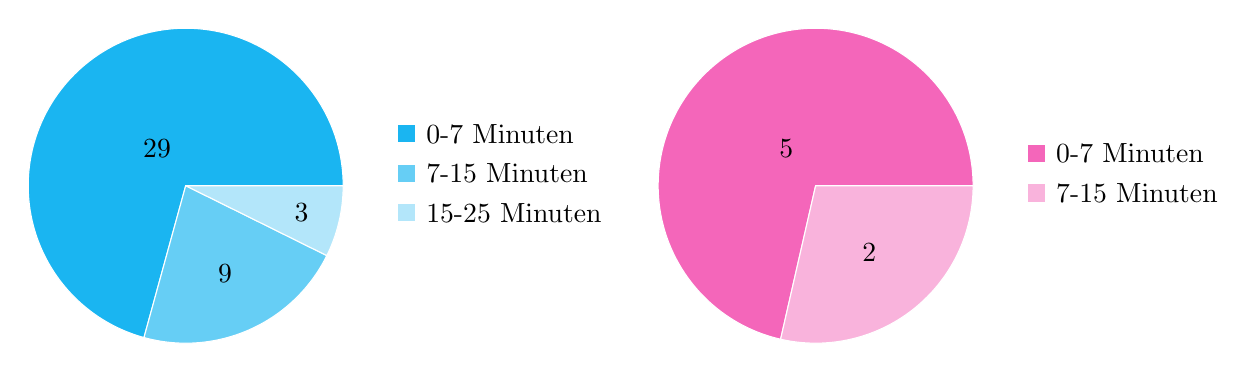
\begin{tikzpicture}
\tikzset{lines/.style={draw=white},}
\pie[color={cyan!90, cyan!60, cyan!30},radius = 2 ,sum=auto, after number=,text=legend,every only number node/.style={text=black},style={lines}]{29/0-7 Minuten,9/7-15 Minuten,3/15-25 Minuten}


\tikzset{lines/.style={draw=white},}
\pie[pos={8,0},radius = 2, color={magenta!60, magenta!30},sum=auto, after number=,text=legend,every only number node/.style={text=black},style={lines}]{5/0-7 Minuten,2/7-15 Minuten}
\end{tikzpicture}
\caption{Links: hatten Spaß. Rechts: hatten \textit{keinen} Spaß}
\end{figure}

	
\section{Referenzen}
\todo{Autor: Svenja}
	Yo
	
\section{Appendix} % = Anhang
\todo{Autor: Svenja}
	Anhang mit Lizenzen usw.
	
\vfill %Zum Seitenende Verschieben

\printbibliography

\end{document}
